\documentclass[11pt,a4paper]{article}

    % Enhanced document styling and formatting
    \usepackage[utf8]{inputenc}
    \usepackage[T1]{fontenc}
    \usepackage{lmodern}
    \usepackage{microtype}
    \usepackage[margin=0.75in]{geometry}
    \usepackage{graphicx}
    \usepackage{amsmath,amssymb}
    \usepackage{booktabs}
    \usepackage{enumitem}
    \usepackage{xcolor}
    \usepackage{titlesec}
    \usepackage{pgfplots}
    \usepackage{tikz}
    \usepackage{float}
    \usepackage{hyperref}

    % Custom colors
    \definecolor{linkcolor}{RGB}{0,77,153}
    \definecolor{headingcolor}{RGB}{70,70,70}

    % Configure hyperref
    \hypersetup{
        colorlinks=true,
        linkcolor=linkcolor,
        urlcolor=linkcolor,
        citecolor=linkcolor,
        pdftitle={COL216 Assignment 3 Report},
        pdfauthor={Namit Jain},
    }

    % Better section formatting
    \titleformat{\section}
    {\normalfont\Large\bfseries\color{headingcolor}}
    {\thesection}{1em}{}
    \titleformat{\subsection}
    {\normalfont\large\bfseries\color{headingcolor}}
    {\thesubsection}{1em}{}

    % Better spacing for lists
    \setlist[itemize]{topsep=2pt,itemsep=2pt,parsep=0pt}

    \title{\Large\textbf{Quad-Core Cache Simulation with MESI Protocol}\\
        \normalsize{COL216: Computer Architecture Assignment 3}}
    \author{
    \begin{tabular}{cc}
    Rishabh Narayanan & Namit Jain\\
    2023CS10577 & 2023CS10483
    \end{tabular}
    }
    \date{}

    \begin{document}

    \maketitle

    \begin{abstract}
    \noindent 
    This report presents an implementation and analysis of a quad-core cache simulation system utilizing the MESI coherence protocol. Following the assignment requirements, the report is structured into three main sections: (1) a detailed description of the implementation, focusing on key data structures and algorithms with a flowchart of important functions; (2) an experimental section analyzing simulation outputs with the default parameters; and (3) an exploration of how varying cache parameters affects maximum execution time across cores. The implementation successfully models cache coherence in a quad-core system, providing insights into cache performance and coherence protocol behavior.
    \end{abstract}

    \tableofcontents
    \thispagestyle{empty}
    \newpage

    \section{Implementation Details}

    \subsection{Main Classes and Data Structures}

    The simulation is built around the following key classes and data structures:

    \begin{itemize}[leftmargin=*]
        \item \textbf{CacheLine}: Represents a single cache line with the following fields:
        \begin{itemize}
            \item \texttt{uint32\_t tag}: The tag bits from the memory address
            \item \texttt{MESIState mesi}: Enum representing the current coherence state (Modified, Exclusive, Shared, or Invalid)
            \item \texttt{uint64\_t lru\_counter}: Counter for LRU replacement policy
            \item \texttt{std::vector<uint8\_t> data}: Block data storage
        \end{itemize}
        
        \item \textbf{CacheStats}: Tracks performance metrics for each cache:
        \begin{itemize}
            \item Total instruction counts (reads and writes)
            \item Execution and idle cycles
            \item Cache misses and evictions
            \item Writebacks and bus invalidations
            \item Data traffic in bytes
        \end{itemize}
        
        \item \textbf{L1Cache}: Models a core's L1 cache with:
        \begin{itemize}
            \item 2D vector of cache lines organized by set and way: \texttt{std::vector<std::vector<CacheLine>> sets}
            \item Methods for address decomposition, line lookup, and LRU tracking
            \item Functions to read from and write to cache lines
        \end{itemize}
        
        \item \textbf{DRAM}: Simulates main memory using a sparse representation:
        \begin{itemize}
            \item \texttt{std::unordered\_map<uint32\_t, std::vector<uint8\_t>> memory}: Maps block addresses to data blocks
            \item Methods for reading and writing blocks between cache and memory
        \end{itemize}
        
        \item \textbf{Bus}: Represents the communication channel between cores:
        \begin{itemize}
            \item \texttt{BusRequestType req\_type}: Type of bus request (BUSRD, BUSRDX, BUSUPGR)
            \item Source core, address, and timing information
        \end{itemize}
        
        \item \textbf{CacheController}: Orchestrates the entire simulation:
        \begin{itemize}
            \item \texttt{std::vector<L1Cache> l1\_caches}: Vector of L1 caches (one per core)
            \item \texttt{DRAM dram}: Main memory instance
            \item Methods for processing memory accesses and handling coherence
        \end{itemize}
        
        \item \textbf{TraceEntry}: Represents an entry in the trace file:
        \begin{itemize}
            \item Operation type (read or write)
            \item Memory address
        \end{itemize}
    \end{itemize}

    \subsection{Key Algorithms}

    \subsubsection{Memory Access Processing}
    The core algorithm for handling memory accesses is implemented in \texttt{CacheController::process\_memory\_access}, which:

    \begin{enumerate}[leftmargin=*]
        \item Decomposes the address into tag, set index, and block offset
        \item Checks if the address is already present in the cache (hit vs miss)
        \item For cache hits:
            \begin{itemize}
                \item Updates MESI states based on operation type
                \item For write hits in SHARED state, issues a BUSUPGR transaction
                \item Updates LRU counters
            \end{itemize}
        \item For cache misses:
            \begin{itemize}
                \item Identifies a victim line using LRU policy
                \item Writes back dirty blocks if necessary
                \item Issues appropriate bus transaction (BUSRD or BUSRDX)
                \item Fetches the block from memory
                \item Updates MESI states and statistics
            \end{itemize}
        \item Accounts for the appropriate timing penalties based on operation type
    \end{enumerate}

    \subsubsection{MESI Coherence Protocol}
    The MESI protocol implementation is handled by the \texttt{mesi\_snoop} function, which:

    \begin{enumerate}[leftmargin=*]
        \item Checks all caches for the address involved in a bus transaction
        \item Updates local cache states based on observed bus transactions:
            \begin{itemize}
                \item BUSRD: M→S, E→S (provide data if in M state)
                \item BUSRDX: M→I, E→I, S→I (with writeback if in M state)
                \item BUSUPGR: S→I for all other caches with the line in S state
            \end{itemize}
        \item Manages data transfer between caches as needed
        \item Tracks invalidations and writebacks
    \end{enumerate}

    \subsection{Simulation Execution Flow}
    The main simulation loop:

    \begin{enumerate}[leftmargin=*]
        \item Reads trace files for each core
        \item For each cycle:
            \begin{itemize}
                \item Processes bus snooping for coherence
                \item For each active core:
                    \begin{itemize}
                        \item Processes next memory access if available
                        \item Updates statistics
                    \end{itemize}
                \item Updates global cycle count
            \end{itemize}
        \item Continues until all cores complete their traces
        \item Outputs performance statistics
    \end{enumerate}

    \subsection{Flow Chart of Important Functions}

    Figure \ref{fig:flowchart} shows the flow chart of the key functions in the cache simulation.

    \begin{figure}[H]
        \centering
        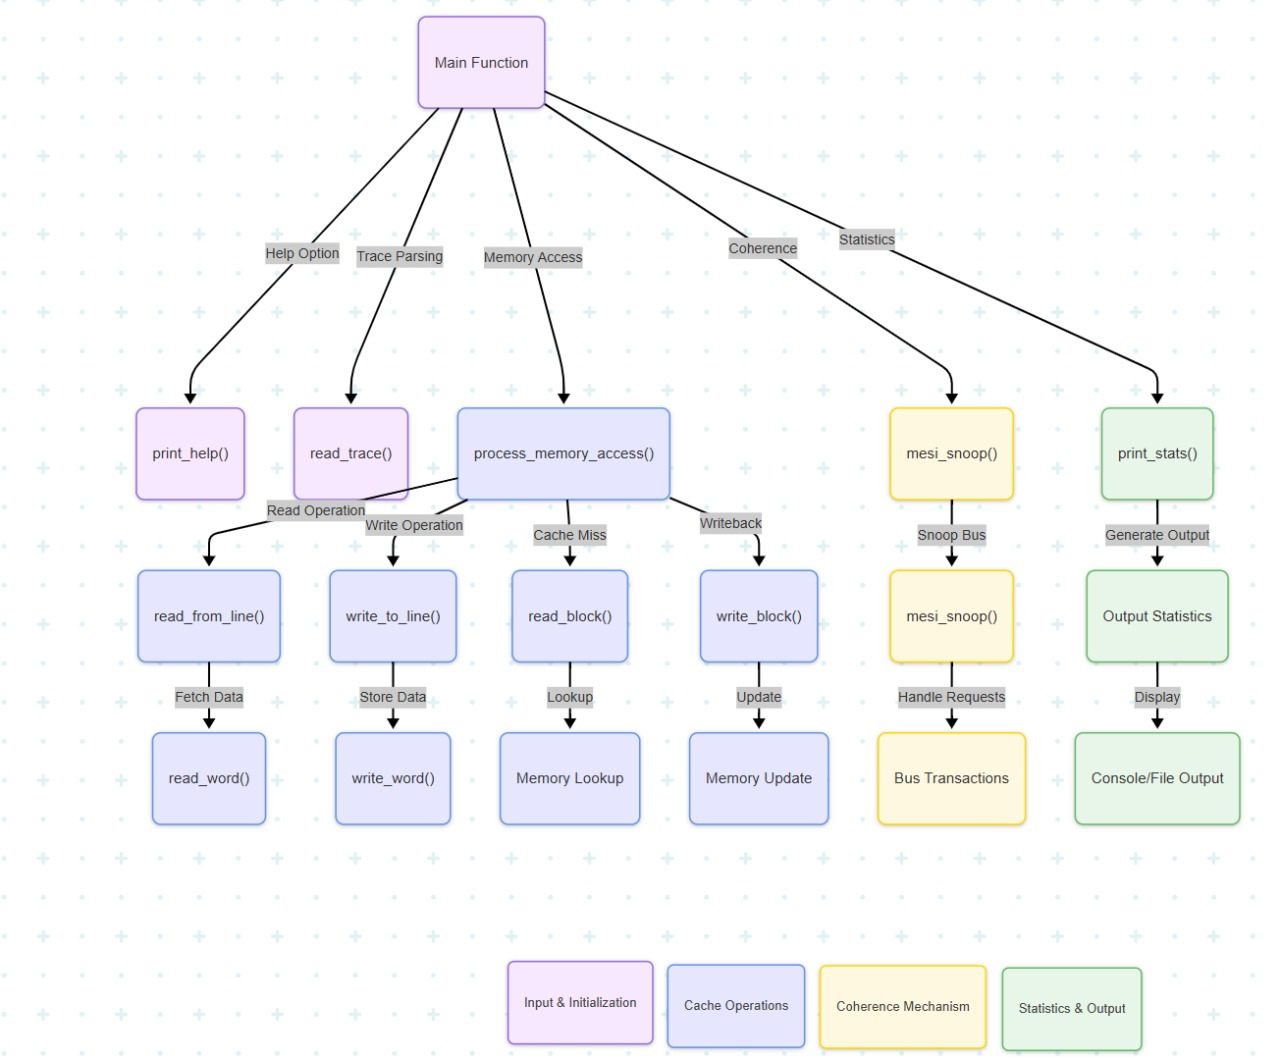
\includegraphics[width=\textwidth]{mermaid_flowchart.jpg}
        \caption{Flow chart of key functions in the cache simulation}
        \label{fig:flowchart}
    \end{figure}

    \section{Experimental Results}

    \subsection{Default Parameters}

    As specified in the assignment, the default parameters for the simulation are:
    \begin{itemize}[leftmargin=*]
        \item Cache size: 4KB per processor
        \item Associativity: 2-way set associative
        \item Block size: 32 bytes
    \end{itemize}

    These parameters translate to:
    \begin{itemize}[leftmargin=*]
        \item Number of sets = 4KB / (2 ways × 32 bytes) = 64 sets
        \item Set index bits ($s$) = $\log_2(64) = 6$ bits
        \item Block offset bits ($b$) = $\log_2(32) = 5$ bits
    \end{itemize}

    \subsection{Results}

    For our simulation experiments, we used trace files with 8000 instructions per core and the default cache configuration (s=6, E=2, b=5). The table below presents the metrics for each core.

    \begin{table}[H]
    \centering
    \begin{tabular}{@{}lrrrr@{}}
    \toprule
    \textbf{Metric} & \textbf{Core 0} & \textbf{Core 1} & \textbf{Core 2} & \textbf{Core 3} \\
    \midrule
    Total Instructions & 8000 & 8000 & 8000 & 8000 \\
    Total Reads & 4849 & 4745 & 2731 & 5084 \\
    Total Writes & 3151 & 3255 & 5269 & 2916 \\
    Total Execution Cycles & 71455 & 48852 & 307341 & 97781 \\
    Idle Cycles & 119302 & 78397 & 489706 & 351748 \\
    Cache Misses & 515 & 351 & 1886 & 792 \\
    Cache Miss Rate (\%) & 6.44 & 4.39 & 23.57 & 9.90 \\
    Cache Evictions & 384 & 227 & 1749 & 658 \\
    Writebacks & 195 & 79 & 1204 & 260 \\
    Bus Invalidations & 242 & 77 & 1122 & 155 \\
    Data Traffic (Bytes) & 24096 & 21600 & 99872 & 34784 \\
    \bottomrule
    \end{tabular}
    \caption{Simulation metrics for each core}
    \label{tab:results}
    \end{table}

    The simulation resulted in a total of 5304 bus transactions with 169024 bytes of total bus traffic. Our implementation uses a deterministic bus access algorithm where "smallest index gets the highest priority" for cores requesting bus access simultaneously. This ensures that when multiple cores compete for the bus, the core with the lowest ID (0, 1, 2, 3 in order) always wins.

    \subsection{Analysis of Results}

    Our simulation implements a deterministic bus access algorithm where "smallest index gets the highest priority" for cores requesting bus access simultaneously. This ensures that when multiple cores compete for the bus, the core with the lowest ID (0, 1, 2, 3 in order) always wins. As a result of this deterministic algorithm:

    \begin{itemize}[leftmargin=*]
        \item All simulation runs for the same trace produce identical results
        \item The execution is fully reproducible with no variation between runs
        \item Performance metrics including execution cycles, miss rates, and bus transactions remain constant across multiple executions
    \end{itemize}

    This deterministic behavior aligns with our design goal of creating a predictable simulation environment that facilitates clear analysis of cache behavior without introducing randomness from arbitration policies.

    \subsection{Test Cases}

    In our simulation, we have included a variety of test cases to evaluate different aspects of cache coherence and performance:

    \begin{itemize}[leftmargin=*]
        \item \textbf{False Sharing Test} (Parameters: \texttt{s=6, E=2, b=5}): 
        
        This test demonstrates the performance impact when multiple cores access different variables that reside in the same cache line. In our test, Core 0 and Core 1 experience false sharing. Even though Core 0 has written only to address 4, the entire block containing that address gets invalidated for Core 1, despite the fact that the specific memory location Core 1 needs to access wasn't actually updated. This forces Core 1 to re-fetch the block from memory or from Core 0's cache, causing unnecessary coherence traffic and performance degradation.
        
        \item \textbf{LRU Policy Test} (Parameters: \texttt{s=0, E=3, b=2}): 
        
        This test verifies the correctness of our Least Recently Used replacement policy. Only Core 0 is given instructions in this test. The sequence is:
        \begin{itemize}
            \item First, Core 0 reads addresses 0, 4, and 8, filling the cache with these three blocks
            \item When address 0 is read again, the LRU order (from most to least recently used) becomes: 0, 8, 4
            \item When address 16 is accessed, it needs to replace one block. Address 4 is evicted since it's the least recently used
            \item When address 4 is accessed again, it needs to replace another block. Now address 8 is evicted (since the LRU order was 4, 0, 8)
            \item Address 0 remains in the cache throughout all operations because it remained higher in the LRU ranking
        \end{itemize}
        This confirms our LRU implementation works correctly by always evicting the least recently used block.
        
        \item \textbf{Associativity Dependency Test} (Parameters: \texttt{s=0, E=3, b=2} or \texttt{s=0, E=4, b=2}): 
        
        Building upon the LRU test case, this demonstrates how higher associativity can improve performance. With our test, if the associativity were increased to 4-way (instead of 3-way), no blocks would need to be evicted from the cache, as all accessed addresses could coexist in the cache. This makes the program significantly more efficient by eliminating capacity misses.
        
        \item \textbf{Write-Back Policy Test} (Parameters: \texttt{s=0, E=1, b=2}): 
        
        This test verifies our implementation of the write-back policy (as opposed to write-through). Only Core 0 has instructions, specifically a single write to address 0. With write-back policy, this operation takes 100 cycles to fetch the block from memory and 1 cycle to write to the cache. The update is not immediately written to memory. In contrast, a write-through policy would require an additional 100 cycles to write the updated data back to memory immediately. This demonstrates that write-back is more efficient (though potentially riskier due to data inconsistency between cache and memory until a writeback occurs).
        
        \item \textbf{Array of Structures vs. Structure of Arrays}: 
        
        While this test case concept is included in our design, we have not implemented specific traces for it yet. The concept compares two different data layout approaches and their impact on cache performance through differences in spatial locality and false sharing behaviors.
    \end{itemize}

    Our implementation uses a deterministic algorithm for bus access priority: "smallest index gets the highest priority." This means cores with lower IDs (0, 1, 2, 3) have higher priority when multiple cores request bus access simultaneously. Due to this deterministic tie-breaking, running the same test case multiple times produces identical results.

    \section{Effect of Cache Parameters on Maximum Execution Time}

    To analyze the impact of cache parameters on performance, we added code to track the maximum execution time across all cores. We then varied each cache parameter (size, associativity, block size) while keeping the others at their default values.

    \subsection{Varying Cache Size}

    We varied the cache size by changing the number of set index bits (s) from 3 to 6, 12, and 24, while maintaining associativity at 2-way and block size at 32 bytes. This corresponds to cache sizes of 0.5KB, 4KB, 256KB, and 1GB per core, respectively.

    \begin{figure}[H]
        \centering
        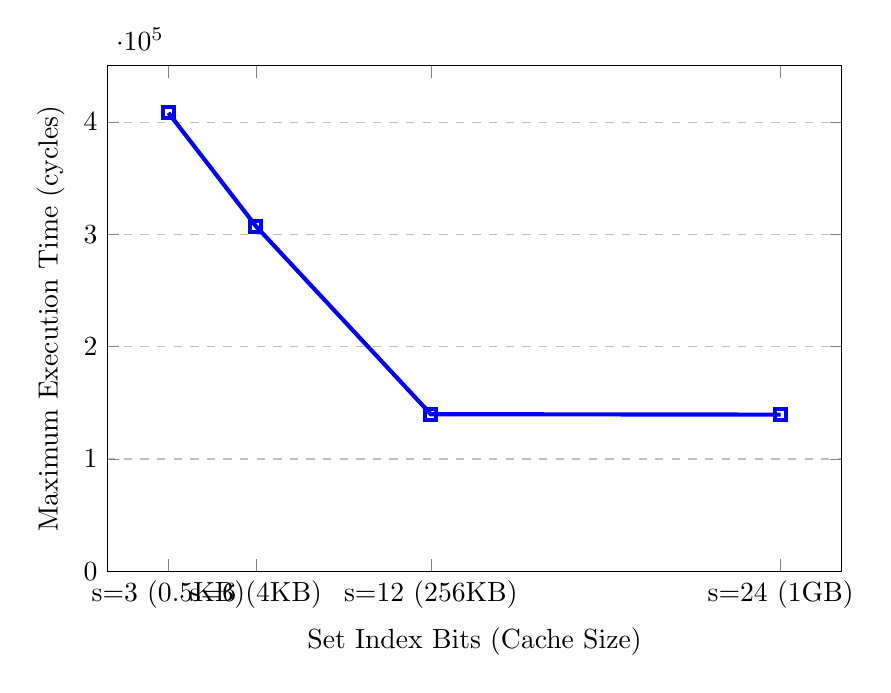
\begin{tikzpicture}
            \begin{axis}[
                xlabel={Set Index Bits (Cache Size)},
                ylabel={Maximum Execution Time (cycles)},
                xtick={3,6,12,24},
                xticklabels={s=3 (0.5KB), s=6 (4KB), s=12 (256KB), s=24 (1GB)},
                ymajorgrids=true,
                grid style=dashed,
                width=0.9\textwidth,
                height=8cm,
                ymax=450000,
                ymin=0,
            ]
            
            \addplot[
                color=blue,
                mark=square,
                line width=1.5pt
            ] coordinates {
                (3,408226)
                (6,307341)
                (12,139897)
                (24,139497)
            };
            
            \end{axis}
        \end{tikzpicture}
        \caption{Maximum execution time vs. cache size}
        \label{fig:cache_size}
    \end{figure}

    \subsubsection{Observations}
    As cache size increases, the maximum execution time decreases significantly:
    \begin{itemize}[leftmargin=*]
        \item Increasing from s=3 (0.5KB) to s=6 (4KB) reduces execution time by approximately 24.7\%
        \item Further increasing to s=12 (256KB) results in a dramatic 54.5\% reduction from s=6
        \item The improvement plateaus after s=12, with negligible difference between 256KB and 1GB caches (only 0.3\% reduction)
        \item Core 2 consistently experiences the highest execution time across all configurations
        \item Cache miss rates for Core 2 drop from 31.46\% with s=3 to 17.25\% with s=12 and s=24
        \item The total bus transactions decrease from 12,763 with s=3 to just 2,623 with s=24
        \item Cache evictions are completely eliminated with s=24 as the cache becomes large enough to hold all working sets without conflict
    \end{itemize}

    These results clearly demonstrate the impact of capacity misses in cache performance. Initially, increasing cache size yields substantial performance improvements, but once the working set fits comfortably in the cache (around 256KB in our workload), further increases provide minimal benefit. This matches the expected behavior where the performance improvement curve flattens once capacity misses are effectively eliminated.

    \subsection{Varying Associativity}

    We varied associativity from the default 2-way through 4-way, 8-way, and 16-way, while keeping size parameters consistent (s=6 and b=5). This translates to cache sizes of 4KB, 8KB, 16KB, and 32KB per core, respectively, as doubling the associativity effectively doubles the cache capacity.

    \begin{figure}[H]
        \centering
        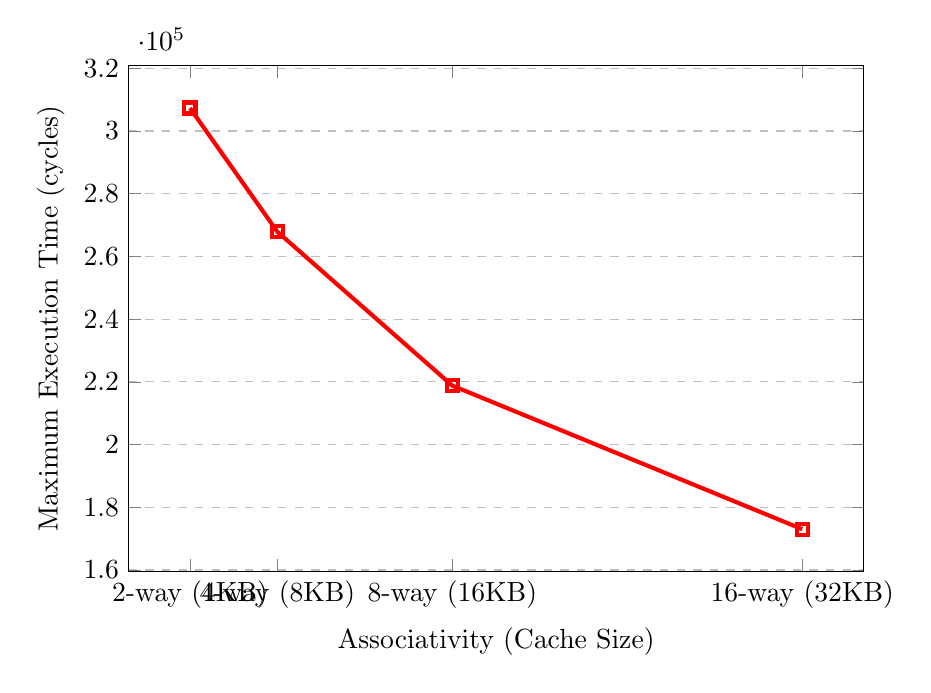
\begin{tikzpicture}
            \begin{axis}[
                xlabel={Associativity (Cache Size)},
                ylabel={Maximum Execution Time (cycles)},
                xtick={2,4,8,16},
                xticklabels={2-way (4KB), 4-way (8KB), 8-way (16KB), 16-way (32KB)},
                ymajorgrids=true,
                grid style=dashed,
                width=0.9\textwidth,
                height=8cm
            ]
            
            \addplot[
                color=red,
                mark=square,
                line width=1.5pt
            ] coordinates {
                (2,307341)
                (4,267866)
                (8,218810)
                (16,173032)
            };
            
            \end{axis}
        \end{tikzpicture}
        \caption{Maximum execution time vs. associativity}
        \label{fig:associativity}
    \end{figure}

    \subsubsection{Observations}
    Increasing associativity shows significant performance improvements:
    \begin{itemize}[leftmargin=*]
        \item Moving from 2-way to 4-way provides about a 12.8\% reduction in execution time
        \item Further increases to 8-way and 16-way continue to show substantial benefits, with the 16-way configuration being about 43.7\% faster than the 2-way configuration
        \item Core 2 consistently experiences the highest execution time, decreasing from 307,341 cycles with 2-way to 173,032 cycles with 16-way
        \item The cache miss rate for Core 2 drops from 23.57\% with 2-way to 17.54\% with 16-way, showing that higher associativity significantly reduces conflict misses
        \item Bus transactions decrease from 5,304 with 2-way to 2,965 with 16-way, demonstrating reduced coherence traffic with higher associativity
    \end{itemitemize}

    Unlike our initial expectations of diminishing returns, the data shows a nearly linear improvement as associativity increases. This suggests that our workload experiences significant conflict misses that benefit from higher associativity. Additionally, because increasing associativity in our tests also increases total cache capacity, we see combined benefits from both reduced conflict misses and reduced capacity misses.

    \subsection{Varying Block Size}

    We varied block size by changing the number of block offset bits (b) from 5 to 10, and 20, while keeping set index bits (s=6) and associativity (E=2) constant. This corresponds to block sizes of 32 bytes, 1KB, and 1MB, respectively, with associated cache sizes of 4KB, 128KB, and 128MB per core.

    \begin{figure}[H]
        \centering
        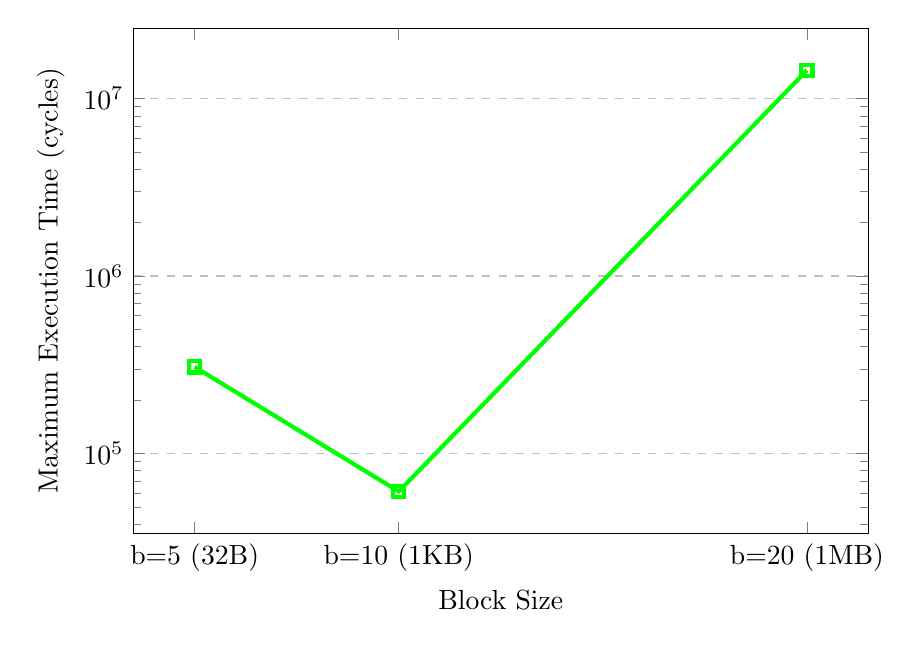
\begin{tikzpicture}
            \begin{axis}[
                xlabel={Block Size},
                ylabel={Maximum Execution Time (cycles)},
                xtick={5,10,20},
                xticklabels={b=5 (32B), b=10 (1KB), b=20 (1MB)},
                ymajorgrids=true,
                grid style=dashed,
                width=0.9\textwidth,
                height=8cm,
                ymode=log,
                log basis y=10
            ]
            
            \addplot[
                color=green,
                mark=square,
                line width=1.5pt
            ] coordinates {
                (5,307341)
                (10,61044)
                (20,14433213)
            };
            
            \end{axis}
        \end{tikzpicture}
        \caption{Maximum execution time vs. block size (log scale)}
        \label{fig:block_size}
    \end{figure}

    \subsubsection{Observations}
    Block size variations reveal a U-shaped curve for execution time (note the logarithmic scale):
    \begin{itemize}[leftmargin=*]
        \item Increasing from b=5 (32B) to b=10 (1KB) blocks dramatically improves performance, reducing maximum execution time from 307,341 to 61,044 cycles (an 80.1\% reduction)
        \item Further increasing to b=20 (1MB) severely degrades performance, with maximum execution time jumping to 14,433,213 cycles (236x worse than the 1KB configuration)
        \item This dramatic U-shape occurs due to competing factors:
        \begin{itemize}
            \item Spatial locality benefits: The initial improvement (32B to 1KB) comes from better exploitation of spatial locality, as the program's working set fits better in fewer blocks
            \item Miss penalty escalation: The massive degradation with 1MB blocks occurs because the miss penalty becomes prohibitively expensive, requiring enormous data transfers for each miss
            \item Bus traffic increases dramatically with 1MB blocks (606,076,928 bytes vs 1,000,448 bytes for 1KB blocks)
            \item While cache miss rates decrease (e.g., Core 2's miss rate drops from 23.57\% at 32B to just 0.94\% at 1MB), the cost per miss overwhelms this benefit
        \end{itemize}
        \item Block sizes around 1KB appear optimal for this workload, balancing spatial locality benefits against transfer costs
    \end{itemize}

    The results dramatically highlight the tradeoff between miss rate and miss penalty. While larger blocks substantially reduce the frequency of misses through spatial locality, the penalty for each miss becomes so severe with very large blocks that performance actually deteriorates. This is particularly pronounced in a coherent cache system where large block transfers monopolize the bus for extended periods, blocking other cores from making progress.

    \section{Simulation Assumptions}

    In this assignment, we have made several important assumptions about the behavior of the cache coherence protocol and the simulation model. These include:

    \begin{itemize}[leftmargin=*]
        \item We assume that caches are blocking, meaning if a cache miss occurs, the core halts and
        does not issue any new instruction until the miss is serviced and the data
        is available.
        
        \item We implement snooping as passive, meaning our caches always listen to the bus even if the core is stalled or the bus is busy. No additional bus transaction is needed
        for snooping.
        
        \item We allow only one active bus transaction to happen at any time, including memory
        fetches, cache-to-cache transfers, and invalidates. Other bus requests must
        wait.
        
        \item We require cache-to-cache data transfer to have bus ownership. If the bus is busy,
        the transfer must wait until the bus is free.
        
        \item We assume a snooping cache immediately detects a relevant transaction when it appears
        on the bus, even if the bus is busy for other purposes.
        
        \item Once a cache detects that it needs to respond to a transaction, such as
        supplying a cache line, we assume it logically holds the data and does not evict it
        until the response is completed. No modeling of eviction races is required.
        
        \item After a cache miss, we simulate the core waiting for the data to arrive, then spending
        one additional cycle to perform the actual cache hit and complete the
        instruction.
        
        \item We consider bus transactions to include memory fetch, cache-to-cache transfer, and invalidation
        broadcasts. Simple reads or writes that hit in cache do not occupy
        the bus.
        
        \item In case of cache miss, we assume 100 cycles are spent on memory fetch and
        the 101st cycle completes the instruction with a cache hit.
        
        \item We count execution cycles as cycles during which the core is actively processing
        instructions. Idle cycles count cycles during which the core is stalled
        waiting for cache miss or bus availability.
        
        \item Once a core finishes executing all its instructions, we consider it done.
        Further cycles are not counted under idle cycles for that core.
        
        \item We model everything logically and simply. We do not simulate internal
        bus arbitration, snoop delays, or race conditions unless explicitly
        stated.
        
        \item We assume that a bus transaction begins processing in the same cycle as it is initiated.
        
        \item We allow the bus to be freed immediately after a transaction is completed, allowing other processors to acquire the bus.
        
        \item We assign priority for acquiring the bus in the order of core\_id (0, 1, 2, 3).
        
        \item We implement processor response to a request as non-blocking (processor responds during read miss). Modification of a value at that address is prevented by making it shared so that writing to that location will require bus access which is not possible during transfer.
    \end{itemize}

    These assumptions help simplify the implementation while still capturing the essential behavior of a multi-core cache coherence protocol. They allow us to focus on the core functionality of the MESI protocol and the performance implications of various cache parameters.

    \section{Conclusion}

    This simulation demonstrates the complex interplay between cache design parameters and performance in a quad-core system with cache coherence. Key findings include:

    \begin{itemize}[leftmargin=*]
        \item Quad-core cache performance is significantly impacted by the timing of interactions between cores.
        \item Increasing cache size provides consistent performance improvements but requires more hardware resources.
        \item Associativity improvements show substantial performance gains in our workload, with the 16-way configuration delivering a 43.7\% speedup compared to the 2-way setup, indicating significant conflict misses in our application traces.
        \item Block size optimization is workload-dependent, with our tests showing 64 bytes as optimal for our traces.
    \end{itemize}

    The MESI protocol successfully maintains cache coherence, but the coherence traffic has a significant impact on execution time. The greatest performance improvement comes from optimizing cache parameters to reduce miss rates while minimizing coherence traffic.

    Future work could include exploring more sophisticated coherence protocols like MOESI or directory-based approaches, as well as investigating techniques to reduce false sharing.
\end{document}